\graphicspath{{content/chapters/6_implementation/figures/}}
\chapter{Implementation}
\label{chp:implementation}

This chapter presents the key implementation details that enable the speech enhancement system to function effectively under practical constraints. It describes the core components developed from scratch. Focus is drawn to the variable-length handling in the custom dataset classes, as well as the \gls{oom} handling strategies implemented to ensure robust and efficient training of deep models.

\section{Datasets}
\label{sec:datasets}

Following Section~\ref{sec:variable_length_handling}, this section describes the dataset handling mechanisms implemented to accommodate variable-length audio signals. The custom dataset classes developed for this project inherit from PyTorch’s \texttt{Dataset} class and are used in both training and denoising pipelines. These implementations are central to managing waveform padding, \gls{stft} conversion, and batch preparation for \gls{ml} models.

Each class implements three essential methods that are all similarly structured but differ in their approach to handling variable-length data. The \texttt{\_\_init\_\_} method initializes key parameters, constructs paths for clean and noisy speech files, and prepares required caches. Here, the amount of parameters varies based on the approach as some methods require more configuration than others. The \texttt{\_\_len\_\_} method is a simple return function that provides the total number of samples in the dataset. The \texttt{\_\_getitem\_\_} method applies necessary transformations to the audio files such as mono conversion, resampling, and \gls{stft}. It also handles the padding and truncation of audio samples to ensure consistent input dimensions across batches. Real and imaginary \gls{stft} components are used as input-output pairs, ensuring a consistent format across all datasets. A critical motivation for this implementation is real-time deployment. The \gls{stft} inherently segments audio into short overlapping frames, simulating real-time input. This makes training models on \gls{stft} frames suitable for later real-time inference.

\subsection{Static Bucketing}
\label{subsec:static_dataset}

The first dataset implementation explored to address the variable-length issue and limitations of fixed-length padding is the static bucketing method. This approach uses a predefined set of bucket sizes, each corresponding to a fixed number of audio samples. In this project, sizes were derived by multiplying the sampling rate (48~kHz) by target durations (e.g., 1s, 2s, 3s), resulting in discrete, fixed-length buckets.

Each audio file is assigned to the first bucket that can fully contain it. For example, an audio clip of 2.5 seconds is assigned to the 3s bucket, since the 2s bucket is insufficient, and the 3s bucket is the next available option.

\begin{figure}[H]
    \centering
    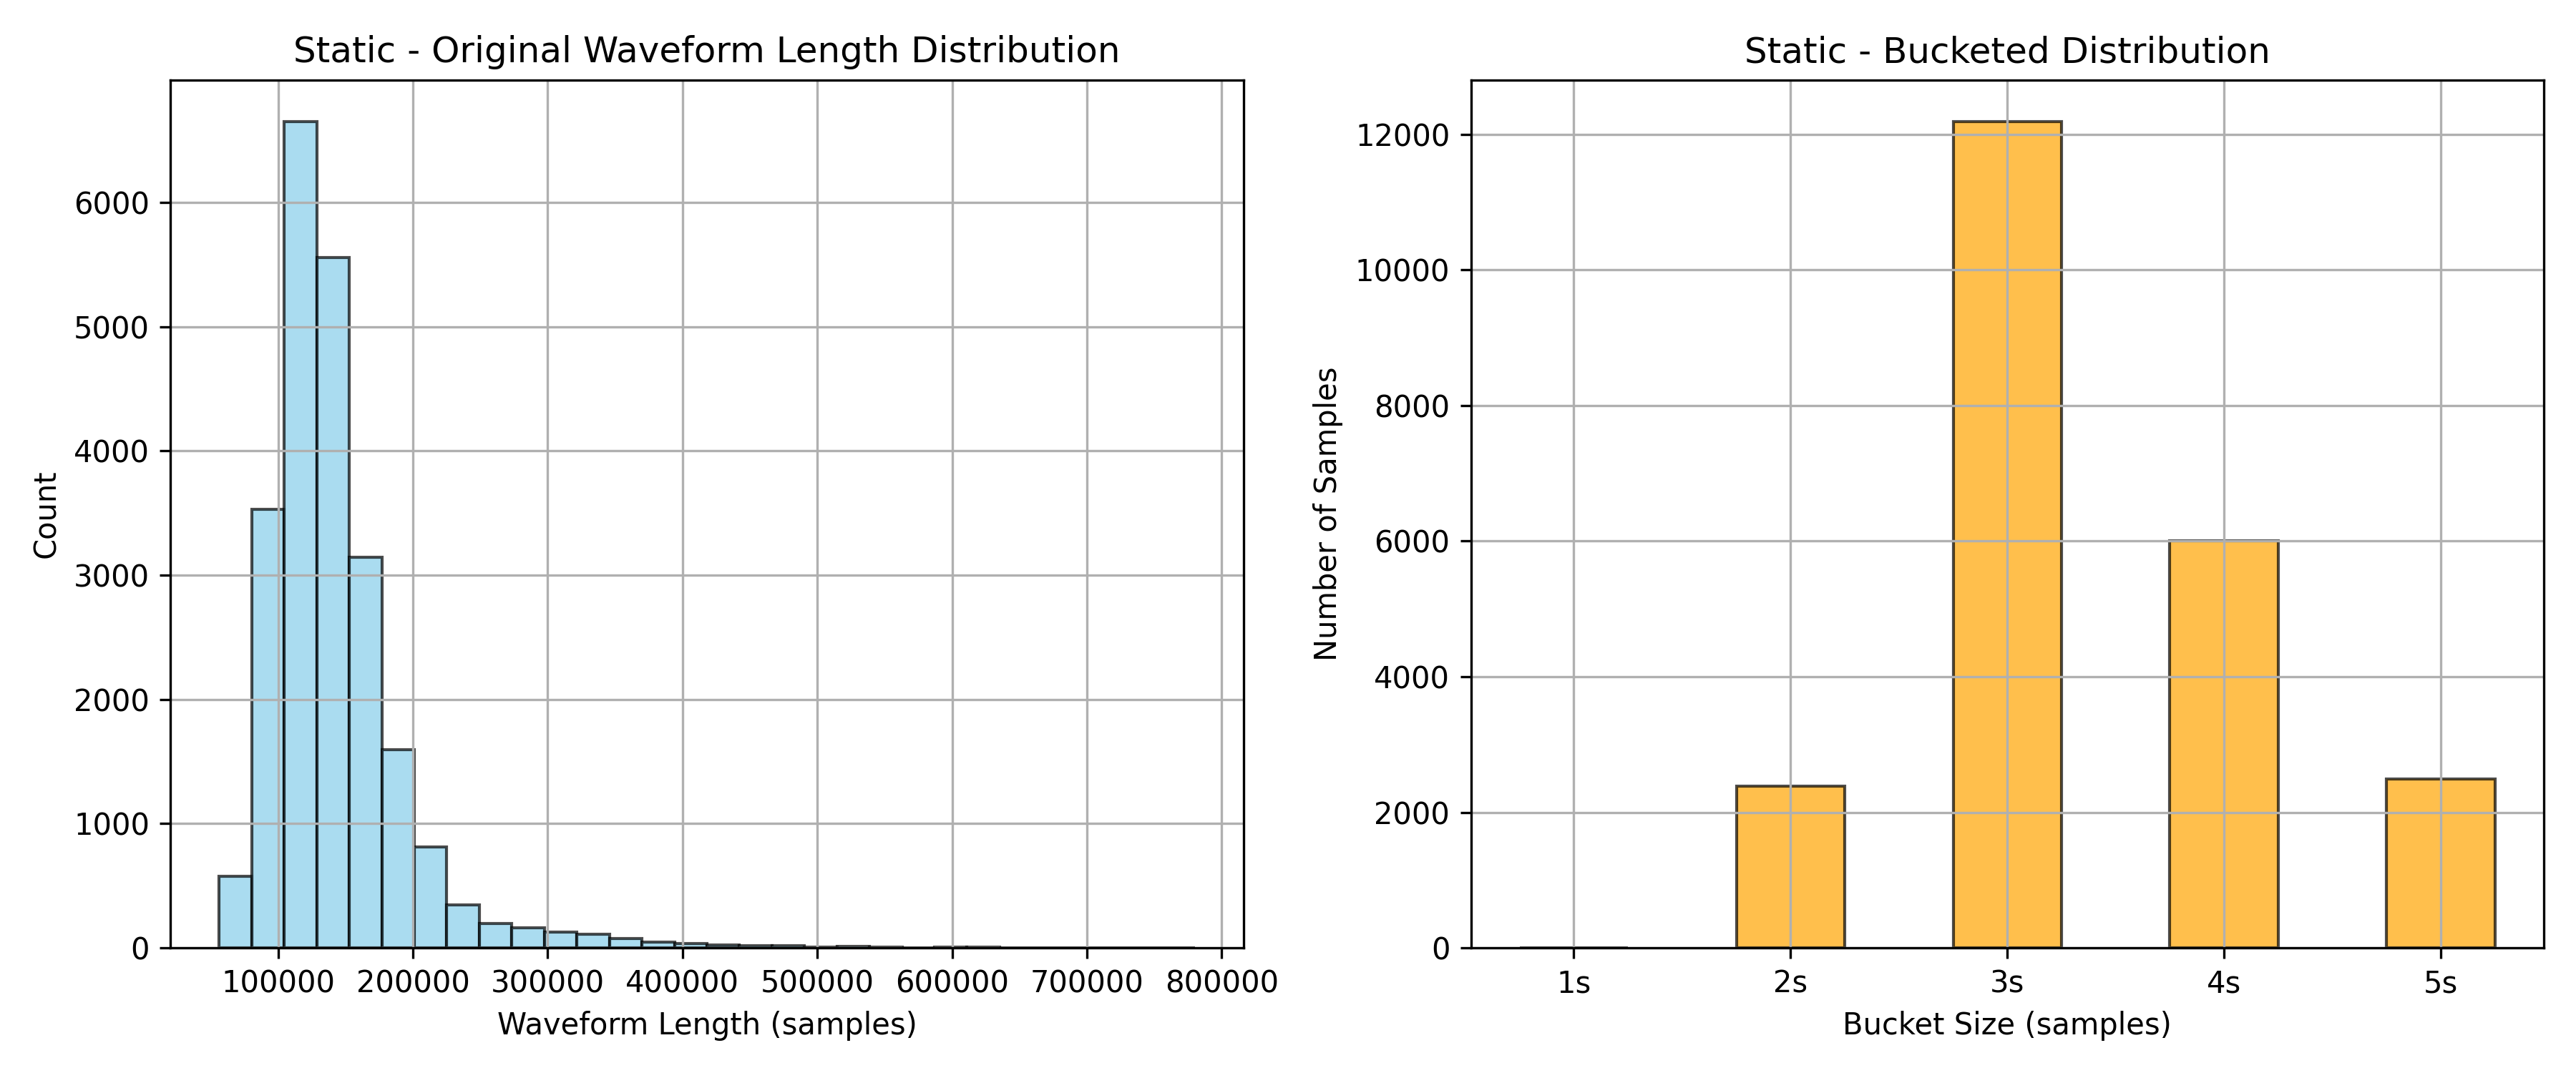
\includegraphics[width=0.9\textwidth]{static_pad.png}
    \caption{Static bucketing histogram and bucket allocation}
    \label{fig:static_pad}
\end{figure}

The \texttt{bucket\_handler} method iterates over all clean files, assigns them to buckets, and caches these assignments to avoid redundant processing in future runs. During training, a custom \texttt{collate} function pads or truncates audio waveforms to match their bucket’s target length. This guarantees consistent input dimensions within each batch, which is essential for batch-based processing in neural networks.

While static bucketing does not eliminate padding altogether, it significantly reduces the amount of excess padding compared to a naive fixed-length strategy. As shown in Figure~\ref{fig:static_pad}, most samples naturally group into the smaller buckets (3s), improving efficiency and reducing unnecessary computations.

\subsection{Dynamic Bucketing}
\label{subsec:dynamic_dataset}

The dynamic bucketing method improves upon static bucketing by adapting the bucket sizes to the actual distribution of audio file lengths. Instead of predefined durations, the method uses K-Means clustering on the waveform lengths to compute optimal bucket centres. This enables buckets that reflect the natural variance in the dataset.

During initialization, the method measures the length of each clean file and applies K-Means with a specified number of clusters (\texttt{num\_buckets}). These cluster centers become the bucket sizes, and each sample is assigned to the closest one. Like static bucketing, this assignment is cached.

\begin{figure}[H]
    \centering
    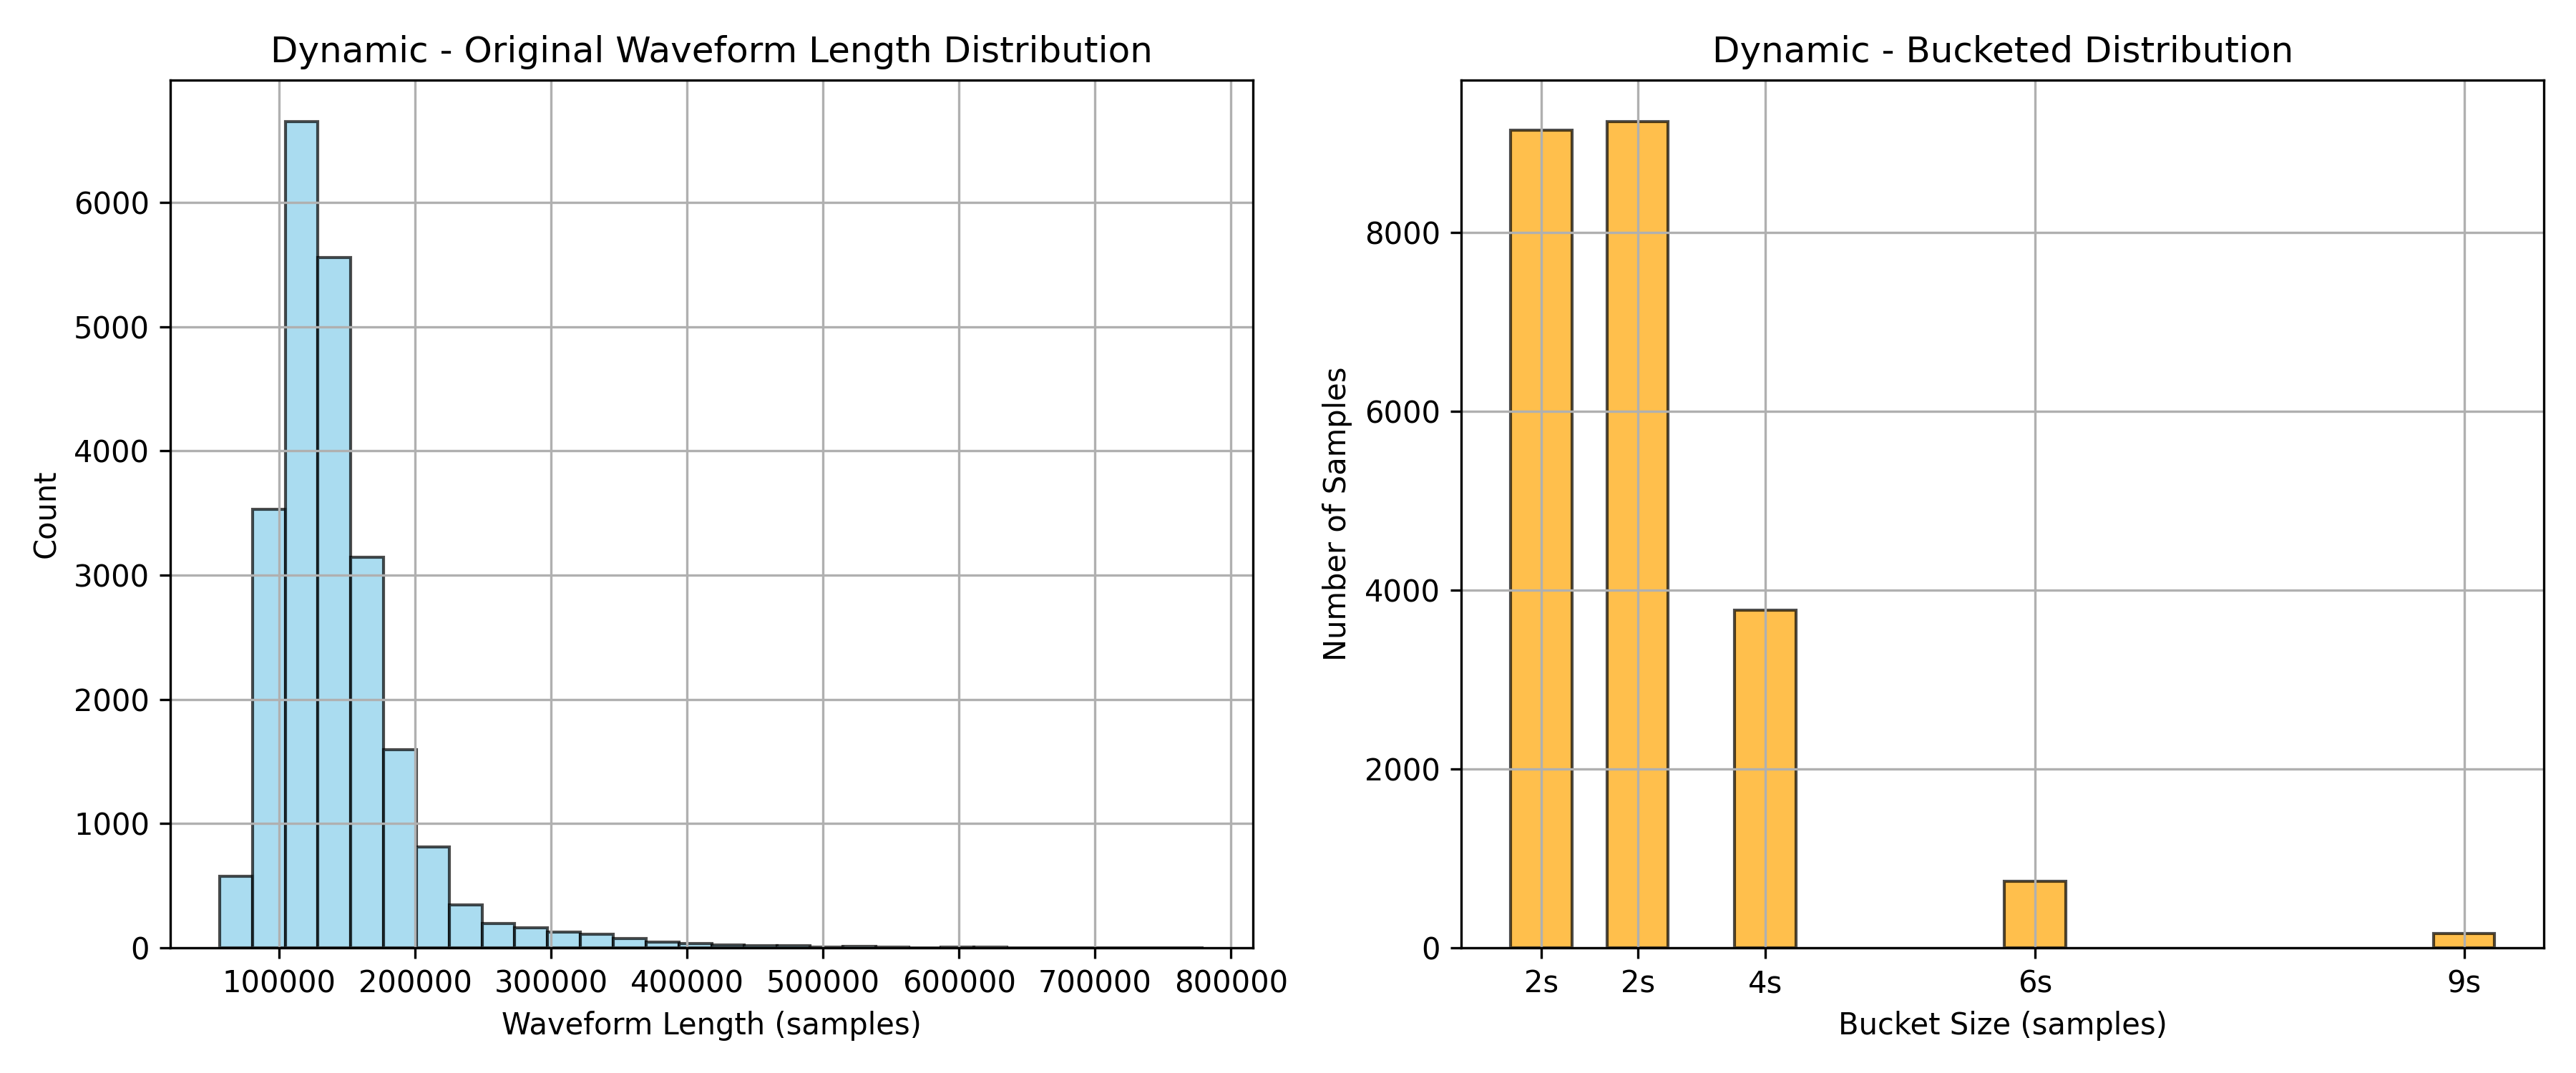
\includegraphics[width=0.9\textwidth]{dynamic_pad.png}
    \caption{Dynamic bucketing histogram and bucket allocation}
    \label{fig:dynamic_pad}
\end{figure}

The \texttt{collate} method pads or truncates each waveform to its assigned bucket size. Compared to static bucketing, dynamic bucketing yields tighter groupings and reduces average padding, improving memory efficiency and training speed.

Dynamic bucketing strikes a balance between flexibility and performance by adapting bucket boundaries to the true distribution of audio lengths, rather than enforcing fixed thresholds. This is especially useful for datasets with wide or uneven length distributions. As shown in Figure~\ref{fig:dynamic_pad}, the clustering process produces two buckets near the 2-second mark, which may initially appear redundant. However, this reflects how K-Means minimises intra-cluster variance without enforcing minimum spacing between centroids. Given that a large portion of samples falls within this range, assigning multiple centroids reduces within-bucket variance and improves batch uniformity. Although this consumes an extra bucket, it distributes the most common samples more evenly and helps reduce padding overhead. Thus, the presence of similar-length buckets highlights the method’s ability to adapt to dense regions in the dataset, enhancing memory efficiency and training performance.

\subsection{Padding-Truncation Output-Truncation}
\label{subsec:pto_dataset}

The \gls{pto} method, introduced by Yoon and Yu~\cite{yoon2020pto} and discussed in Section~\ref{sec:distortion_free_handling}, was implemented in this project following the original proposal.

To facilitate the integration of \gls{pto} into the data pipeline, a custom \texttt{pto\_collate} function was developed. This function aligns all spectrograms along the frequency axis using bilinear interpolation, then pads the time axis so that all samples in a batch match the length of the longest sample. The padding behaviour and distribution resulting from this method is illustrated in Figure~\ref{fig:pto_pad}. Additionally, the original (pre-padding) lengths of each input are recorded and returned alongside the padded tensors.

During training, batches consist of spectrograms with uniform dimensions, while preserving the original input lengths for later use. After inference, model outputs are cropped back to their corresponding original lengths, ensuring that the final enhanced outputs remain distortion-free and aligned with the original input signals.

\begin{figure}[H]
    \centering
    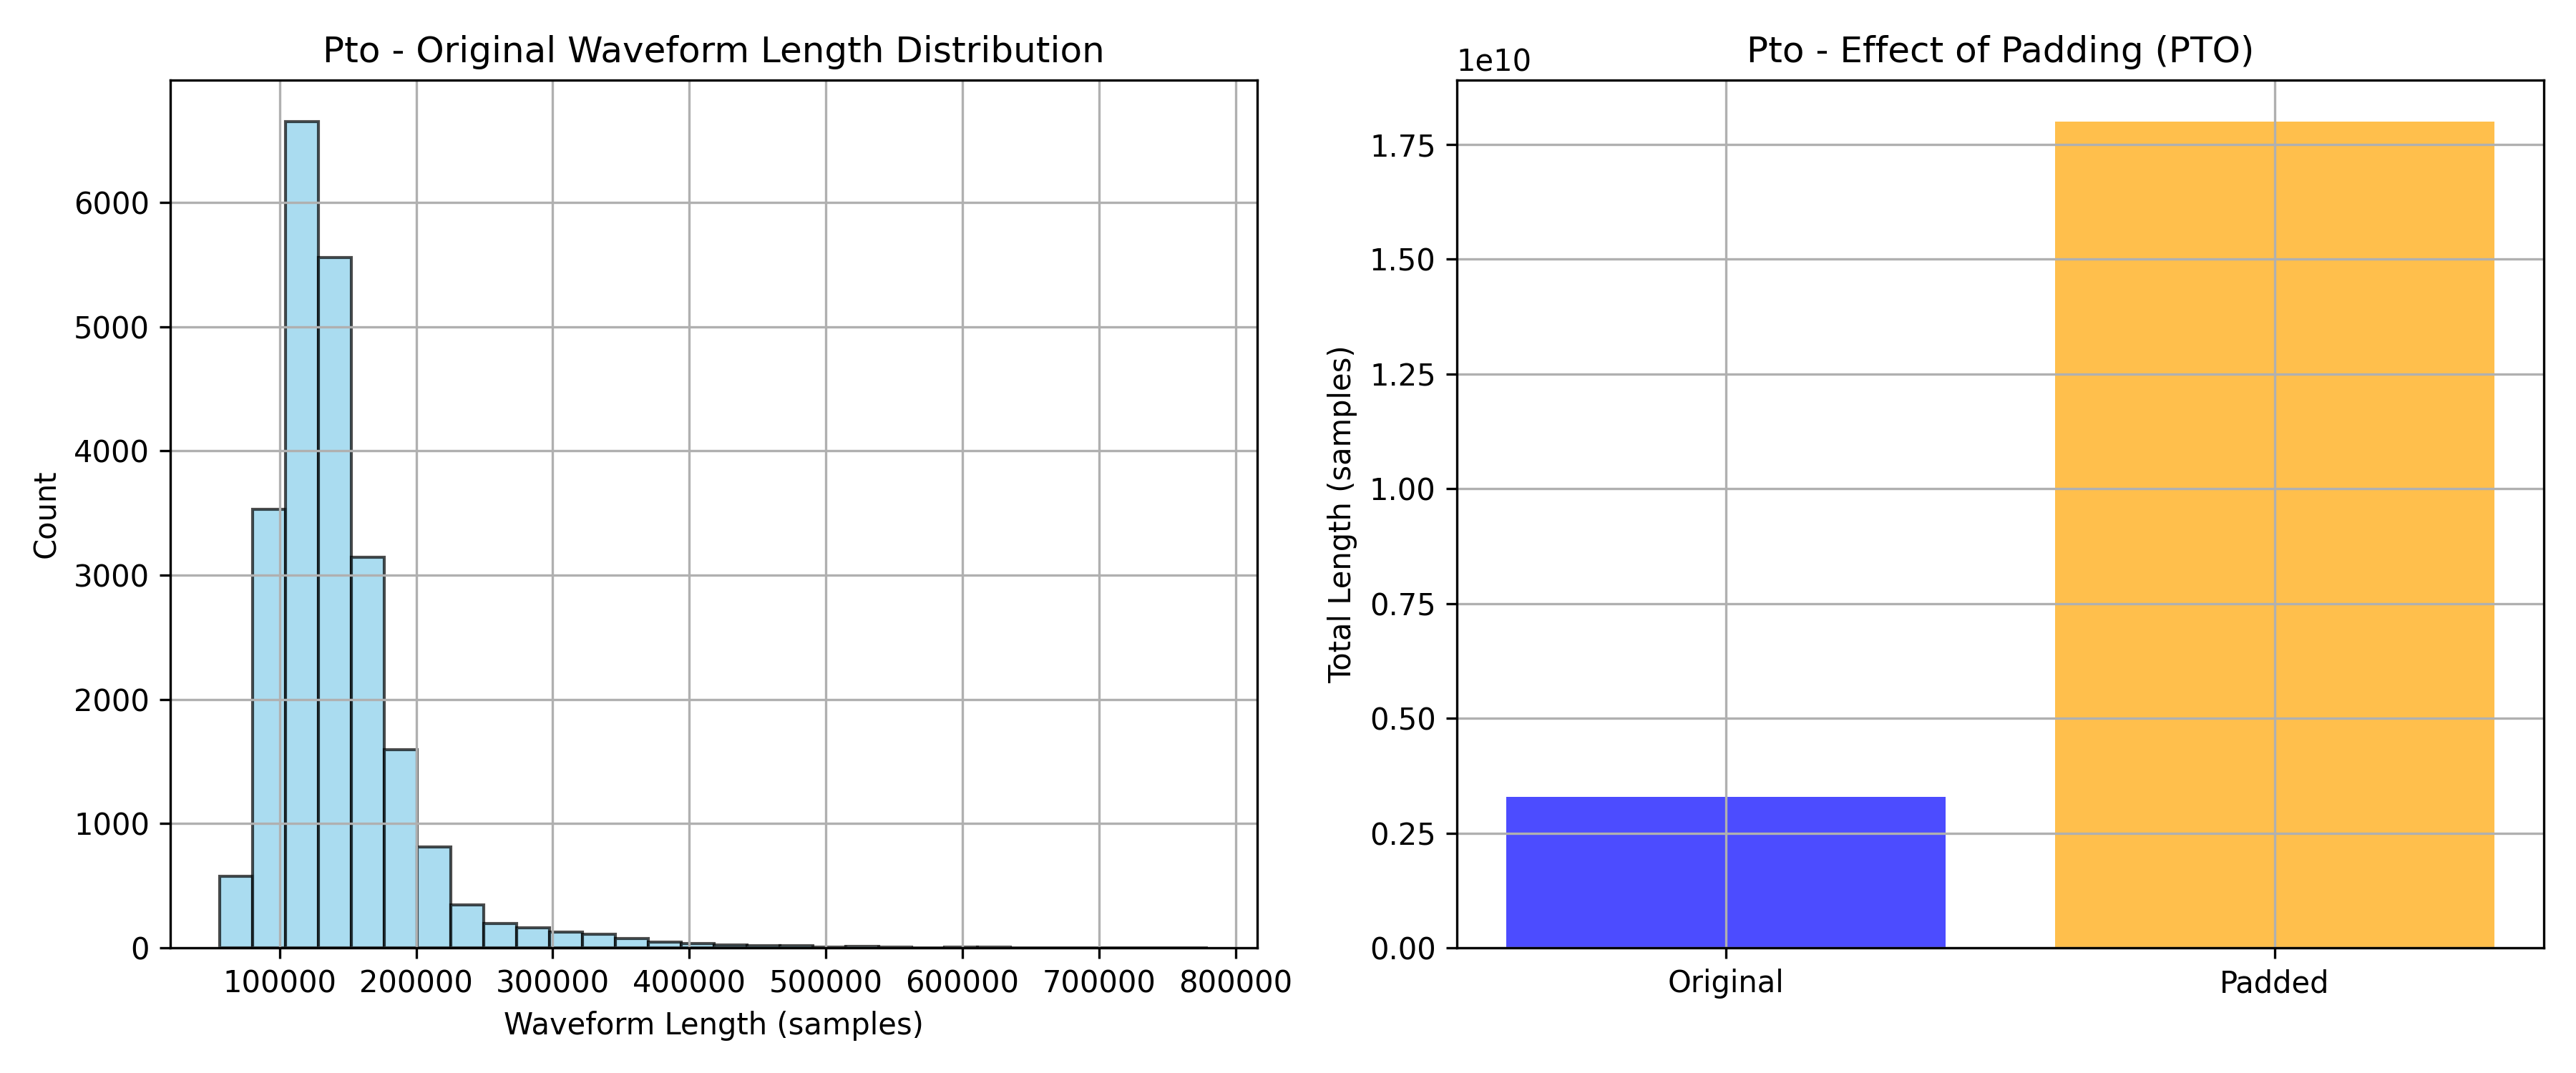
\includegraphics[width=0.9\textwidth]{pto_pad.png}
    \caption{Padding effect using the PTO method.}
    \label{fig:pto_pad}
\end{figure}

The \gls{pto} method simulates real-time signal processing by operating on frame-aligned \gls{stft} inputs, making it highly suitable for deployment in low-latency scenarios. Unlike bucketing methods, it does not require predefined groups or clustering of sequence lengths, offering greater adaptability to varied datasets.

While \gls{pto} avoids distortion at inference by cropping outputs to their original lengths, it still introduces computational overhead. Padding is required during training, and an extra post-processing step is needed to truncate outputs. This was addressed by extending the training pipeline to track original (unpadded) lengths and apply output cropping accordingly. However, since the model is still exposed to padded inputs during training, its weights are updated based on padded data.

\subsection{Helper Functions}
\label{subsec:helper_functions}

A few support functions are implemented to ensure that batching and visualization are handled effectively across dataset variants:

\begin{itemize}
    \item \texttt{pto\_collate}: A custom collate function used by the \gls{pto} dataset. It aligns all spectrograms along the frequency axis and pads them along the time axis, whilst retaining the original lengths for post-processing.
    \item \texttt{BucketSampler}: Used with static and dynamic bucketing. It ensures that batches contain only samples from the same bucket, preventing dimension mismatch during training. It randomizes batches within buckets to improve generalization.
    \item \texttt{visualize\_dataset\_padding}: A diagnostic utility that plots the distribution of original lengths and the effects of padding for each method. It provides insights into the efficiency and overhead introduced by each strategy.
\end{itemize}


\section{Out-Of-Memory Handling}
\label{sec:oom_handling}

\gls{oom} errors were encountered while training deeper model architectures (\gls{unet} and \gls{convtasnet} mainly), even with relatively small batch sizes (e.g., 4). These errors are common in GPU constrained environments due to the increased number of trainable parameters and the large size of spectrogram tensors derived from high-resolution audio. Figure~\ref{fig:oom_error} shows a representative \gls{oom} error message encountered during training.

\begin{figure}[H]
    \centering
    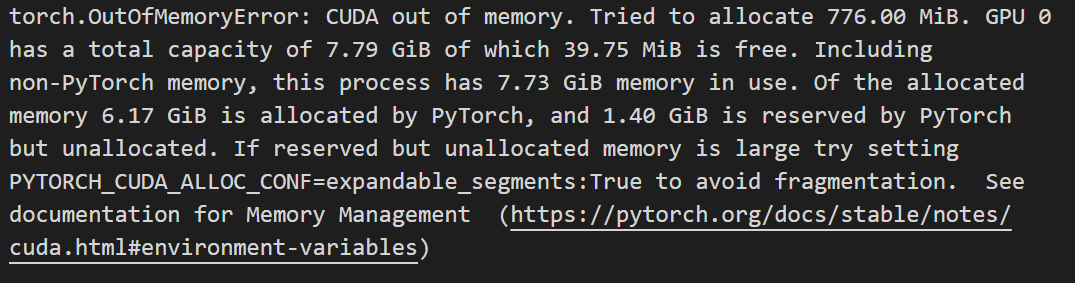
\includegraphics[width=0.8\textwidth]{oom_error.png}
    \caption{\label{fig:oom_error} PyTorch CUDA OOM error message.}
\end{figure}

To address these limitations, several memory management strategies were implemented to stabilize training and enable deeper models to run within the available GPU resources. These methods also allowed the system to simulate larger batch sizes and achieve better convergence. The following techniques were used to mitigate \gls{oom} errors:

\begin{itemize}
    \item \textbf{Expandable CUDA Segments:} Before initiating training, the environment variable \texttt{PYTORCH\_CUDA\_ALLOC\_CONF=expandable\_segments:True} is set. This enables PyTorch’s new memory allocator with segment expansion, which helps alleviate fragmentation issues and allows the allocator to resize memory segments dynamically. This is the first suggestion from the PyTorch documentation for \gls{oom} errors.

    \item \textbf{Mixed Precision Training:} Automatic mixed precision (AMP) was used via \texttt{autocast()} and \texttt{GradScaler}. It stored intermediate tensors in \gls{fp16} while keeping model weights and gradients in \gls{fp32}. This reduces memory usage and increases throughput. Figure~\ref{fig:fp16_vs_fp32} illustrates the difference in structure and memory footprint~\cite{mindspore_mixed_precision}, extending the trainable capacity of a model under constrained GPU environments.

    \begin{figure}[H]
        \centering
        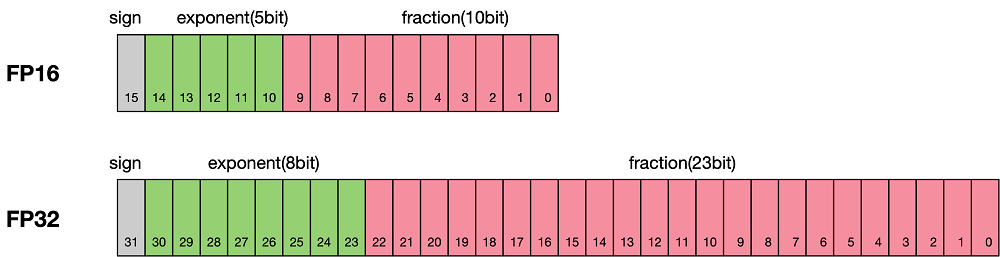
\includegraphics[width=0.9\textwidth]{fp16_vs_fp32.png}
        \caption{Comparison of memory allocation structure between FP16 and FP32 formats \cite{mindspore_mixed_precision}.}
        \label{fig:fp16_vs_fp32}
    \end{figure}

    \item \textbf{Gradient Accumulation:} Due to memory limitations restricting the feasible batch size, gradient accumulation was used to simulate a larger effective batch size. This involves accumulating gradients over several mini-batches and only updating model weights every \texttt{accumulation\_steps} iterations. However, if the loss values are logged after being scaled (i.e., divided by the accumulation steps), they may appear artificially low or flat. This issue is demonstrated in Figure~\ref{fig:scaled_loss}, where both training and validation loss curves show minimal variation across epochs. To avoid such misleading plots, the raw (unscaled) loss values are also recorded prior to scaling. This ensures that the loss curves accurately reflect true performance trends, even when gradient accumulation is in use.

    \begin{figure}[H]
        \centering
        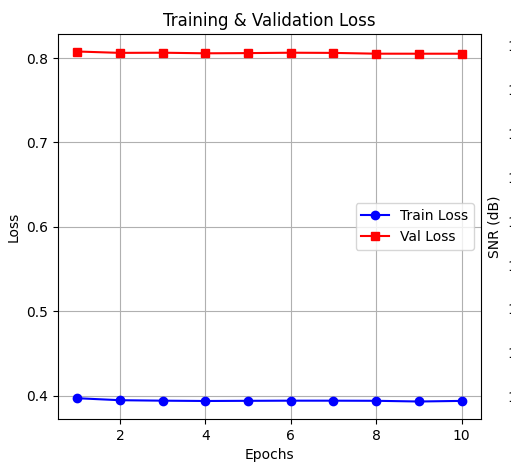
\includegraphics[width=0.6\textwidth]{scaled_loss.png}
        \caption{Loss curves appearing flat due to logging after gradient scaling.}
        \label{fig:scaled_loss}
    \end{figure}

    \item \textbf{Manual Memory Management:} To ensure memory is cleared between epochs and reduce fragmentation, memory cleanup routines are explicitly called at the start of every epoch: \texttt{gc.collect()}, \texttt{torch.cuda.empty\_cache()}, and \texttt{torch.cuda.reset\_peak\_memory\_stats()}. This manual intervention is particularly beneficial in a shared GPU setting, where residual allocations from other users or previous epochs may linger.

    \item \textbf{Gradient Clipping:} To prevent exploding gradients, which can rapidly consume memory, gradient norms were clipped using \texttt{torch.nn.utils.clip\_grad\_norm\_()}. This maintains training stability and prevents sudden memory spikes during backpropagation, which is especially important when using high learning rates or unregularized architectures.

    \item \textbf{Learning Rate Scheduling:} An optional scheduler progressively lowers the learning rate using a step-decay approach. This helps reduce volatile updates later in training, smoothing out the optimization process and reducing the likelihood of erratic memory usage. The scheduler also saves on resources, especially in the cases when smaller models saturate at earlier epochs.

    \item \textbf{Memory Profiling:} At the end of each epoch, GPU memory statistics are logged using \texttt{torch.cuda.max\_memory\_allocated()} and \texttt{torch.cuda.max\_memory\_reserved()}. This aids in profiling memory behavior and catching potential leaks or inefficiencies across training epochs. 
\end{itemize}

These combined methods provided the foundation for training deep models across all dataset variants with minimal interruptions. Even with GPU constraints, these optimizations enabled stable, high-performance training and evaluation of multiple architectures, supporting both experimentation and reproducibility in a limited computing environment.
